%!TEX root = practica.tex
%===============================================================================
\chapter*{Overview}\label{ch:overview}
\addcontentsline{toc}{chapter}{Overview}
%----------------------------------------------------------------------

\section*{Laboratory kit components}
\addcontentsline{toc}{section}{Laboratory kit components}

The laboratory kit includes:
\begin{itemize}
\item	An STM32F407 computer board that emulates an on-board computer (OBC) system.

\item	A USB A / mini USB cable that is used to connect the OBC to the development station hosted on the student PC.

\item	A USB / UART interface cable that is used to provide a serial line link between the OBC board and the ground station software running on the student PC.
\end{itemize}

The figure~\ref{fig:kit} shows the components of the laboratory kit and the connections to a PC.

\begin{figure}[h]
            \centering{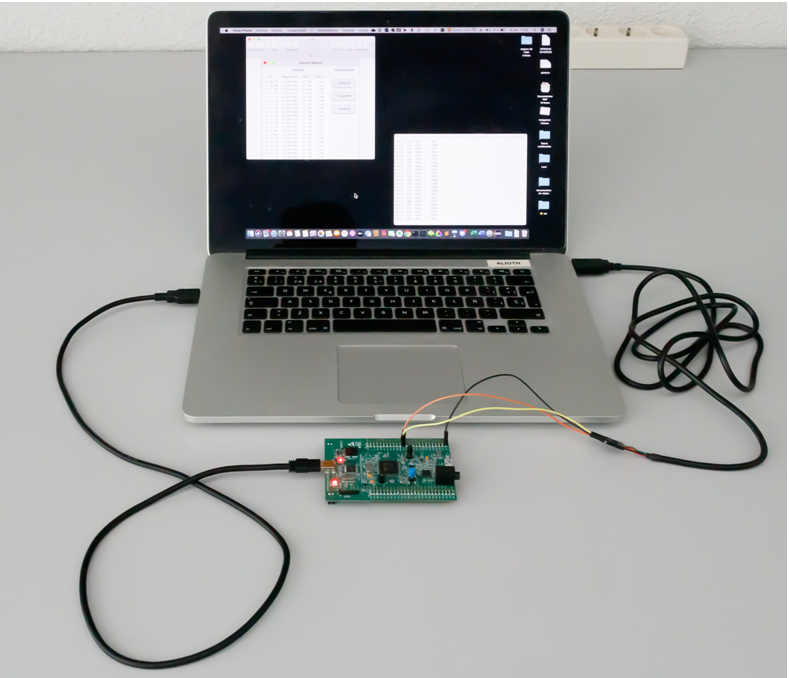
\includegraphics[width=.6\textwidth,keepaspectratio]{laboratory_kit.png}}
            \caption{Laboratory kit.}
            \label{fig:kit}
\end{figure}

\section*{Architecture of the laboratory system}
\addcontentsline{toc}{section}{Architecture of the laboratory system}

The figure~\ref{fig:architecture} depicts the architecture of the laboratory system which consists of two segments.
The \textit{flight segment} is deployed on the laboratory computer board,
and, the \textit{ground segment} is deployed on the student's PC.
The communication between both segments is carried out by means of a serial line,
simulating the radio link of a real satellite mission.
The student's work is centered on programming the computer board.
The ground station software will be provided by the professors.

\begin{figure}[hbtp!]
            \centering{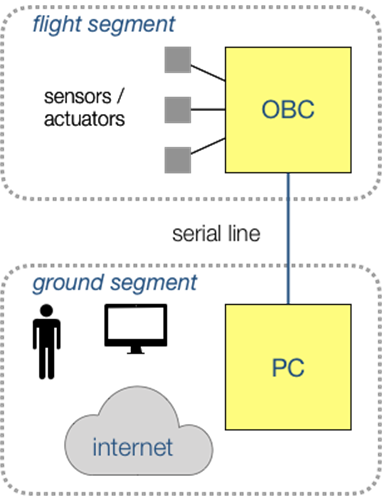
\includegraphics[width=0.35\textwidth,keepaspectratio]{architecture.png}}
            \caption{Architecture of the laboratory system.}
            \label{fig:architecture}
\end{figure}

\section*{Computer board and connections}
\addcontentsline{toc}{section}{Computer board and connections}

The STM32F407 board is used as a low-cost replacement for a satellite OBC.
The board features a 32-bit ARM Cortex-M4 microcomputer,
192 KB of RAM, 1 MB of Flash memory and a number of embedded devices.
The figure~\ref{fig:board}
shows an overall view of the computer board.

\begin{figure}[h]
    \centering{\includegraphics[height=10.2cm,keepaspectratio]{board-v2.png}}
    \caption{Computer board.}
    \label{fig:board}
\end{figure}

The following are the main components used in this laboratory:
\begin{itemize}
\item	USB ST-LINK connector, which is linked to a PC with a mini-USB to USB-A cable. This connection is used to supply power to the board (5 V) and load and debug the software from the host PC.

\item	General Purpose Input-Output (GPIO) pins PB6, PB7 and GND.
GPIO is a standard interface for connecting external devices.
These GPIO pins are used in the laboratory
to connect a serial line to a USB port on a PC,
emulating the connection to the on-board radio equipment in a satellite.
Specifically the pin:
\begin{itemize}
	\item \textbf{PB6} is used as the transmitter pin (TX).
	\item \textbf{PB7} is used as the receiver pin (RX).
	\item \textbf{GND} is used for grounding.
\end{itemize}

\item	Temperature and voltage sensors. These sensors are part of the STM32 microcomputer chip,
and can be read using internal registers in the MCU.
They are used in the laboratory to emulate the housekeeping devices onboard the satellite.
\end{itemize}
